\documentclass[a4paper,12pt]{article} 

%%% Работа с русским языком
\usepackage{cmap}                           % поиск в PDF
\usepackage{mathtext} 			 	       % русские буквы в формулах
\usepackage[T2A]{fontenc}               % кодировка
\usepackage[utf8]{inputenc}              % кодировка исходного текста
\usepackage[english,russian]{babel}  % локализация и переносы
\usepackage[left=2cm,right=2cm,
    top=2cm,bottom=3cm,bindingoffset=0cm]{geometry}
\usepackage{wrapfig}
\usepackage{gensymb}
\usepackage{textcomp}
\usepackage{multirow}
\usepackage{amsmath,amsfonts,amssymb,amsthm,mathtools} % AMS
\usepackage{euscript}	 % Шрифт Евклид
\usepackage{mathrsfs} % Красивый матшрифт
\usepackage{graphicx}%Вставка картинок правильная
\usepackage{float}%"Плавающие" картинки
\usepackage{wrapfig}%Обтекание фигур (таблиц, картинок и прочего)
\title{Лабораторная работа 3.4.2 

Закон Кюри-Вейсса}
\author{Кагарманов Радмир Б01-106}
\date{27 сентября 2022 г.}

\begin{document}
\maketitle
\thispagestyle{empty}
\newpage
\setcounter{page}{1}

\paragraph{Цель работы:}изучение температурной зависимости магнитной восприимчивости ферромагнетика выше точки Кюри.
\paragraph{В работе используется:}катушка самоиндукции с образцом из гадолиния, термостат, частотомер, цифровой вольтметр, $LC$-автогенератор, термопара медь-константан.
\paragraph{Теория\\}
Вещества с отличным от нуля атомными магнитными моментами обладают парамагнитными свойствами. При повышении температуры $T$ возрастает дезориентирующее действие теплового движения частиц, и магнитная восприимчивость парамагнетиков убывает по \textbf{закону Кюри} - обратно пропорционально температуре:
\begin{equation}
    \chi \propto \frac{1}{T}
\end{equation}\par
Некоторые парамагнетики при понижении температуры испытывают фазовый переход в ферромагнитное состояние. Температуру перехода парамагнетик-ферромагнетик называют \textbf{температурой Кюри} $\Theta_{\text{K}}$. Температурная зависимость магнитной восприимчивости у ферромагнетиков выше точки Кюри с удовлетворительной точностью описывается \textbf{законом Кюри-Вейсса}:
\begin{equation}
    \chi \propto \frac{1}{T-\Theta_{p}},
\end{equation}
где $\Theta_{p}$ - параметр с размерностью температуры, называемый иногда \textbf{парамагнитной точкой Кюри}. Величина $\Theta_{p}$ близка к $\Theta_{\text{K}}$, но не совпадает с ней.
\paragraph{Экспериментальная установка\\}
Схема установки представлена на рис. 1.

\begin{figure}[!h]
\centering
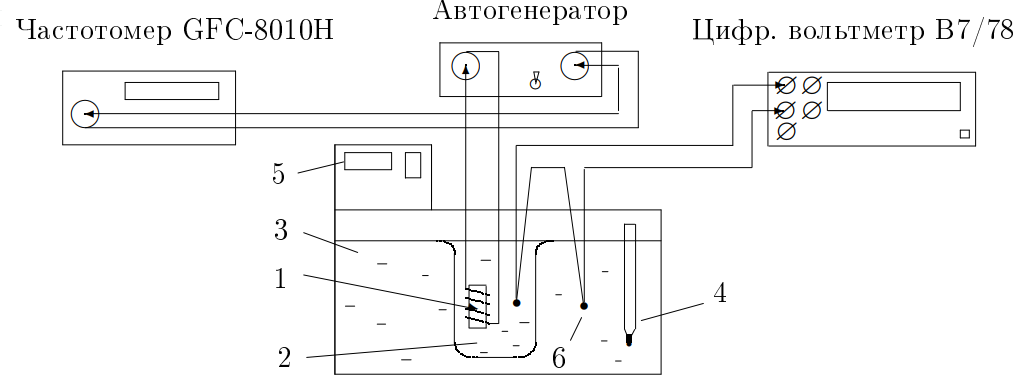
\includegraphics[width=0.9\linewidth]{установка.png}
\caption{Экспериментальная установка}
\label{fig:mpr}
\end{figure}

Катушка 1 с образцом помещена в стеклянный сосуд 2, залитый трансформаторным маслом. Масло предохраняет образец от окисления и способствует ухудшению электрического контакта между отдельными частичками и образца. Кроме того, оно улучшает тепловой контакт между образцом и термостатируемой жидкостью 3 в термостате. Ртутный термометр 4 используется для приближённой оценки температуры.\par
При изменении температуры меняется магнитная восприимчивость образца $\chi$, а следовательно, самоиндукция катушки и период колебаний $\tau$ автогенератора. Для измерения периода используется частотомер.\par
Закон Кюри-Вейсса справедлив, если выполнено соотношение 
\begin{equation}
    \frac{1}{\chi} \sim (T - \Theta_{p}) \sim \frac{1}{(\tau^2 - \tau_{0}^{2})},
\end{equation}
где $\tau_{0}$ - период колебаний в отсутствие образца.\par 
Величина стабилизируемой температуры задаётся на дисплее 5 термостата. Температура исследуемого образца всегда несколько отличается от температуры дистилированной воды в сосуде. Разность температур контролируется с помощью медноконстантановой термопары 6 и цифрового вольтметра. Рекомендуется измерять период колебаний автогенератора в тот момент, когда указанная размерность температур становится $\leq 0,5 \degree C$. Чувствительность термопары $\kappa = 24~ град/мВ$.
\paragraph{Ход работы и обработка результатов}
\subparagraph{1.} Запишем данные установки: $\tau_{0} = 8,252$ мкс, $\delta_{\Delta U} = 0,0012$ мВ.
Так как $\Delta T$ не должно превышать $0,5\degree C$, то максимальное напряжение, при котором можно проводить измерения, равно:
\begin{center}
    $U_{\text{max}}= \frac{\Delta T}{\kappa}\approx 0,021~мВ $ 
\end{center}

Температура образца вычисляется по формуле:
\begin{center}
    $T_{\text{о}} = T_{\text{т}} + \Delta U \cdot \kappa$,
\end{center}
где $T_{\text{т}}$ - температура термостата.\par
Результаты занесём в таблицу 1.

\begin{table}[h!]
\begin{center}
\begin{tabular}{|c|c|c|c|c|c|c|}
\hline
№ & $T_{т},~\degree C$ & $\Delta U$ мкВ & $T_{о}, ~\degree C$ & $\tau$, мкс & $\tau ^{2} - \tau _{0}^{2}, ~ мкс^{2}$ & $\frac{1}{\tau ^{2} - \tau _{0}^{2}}, ~ мкс^{-2}$ \\ \hline
1    & 14   & -13,0            &    13,7       & 10,07           &  33,35           & 0,03           \\ \hline
2    & 16   & -19,3           &    15,6           & 9,96           & 31,11           & 0,03           \\ \hline
3    & 18   & -20,0            & 17,5           & 9,77         & 27,30          & 0,04           \\ \hline
4    & 20   & -17,9            & 19,6         & 9,43           & 20,85            & 0,05           \\ \hline
5    & 21   & -17,6            & 20,6         & 9,23           & 17,17           & 0,06           \\ \hline
6    & 22   & -18,6            & 21,6         & 9,03           & 13,48            & 0,07           \\ \hline
7    & 24   & -18,6            & 23,6         & 8,75           & 8,43            & 0,12           \\ \hline
8    & 26   & -18,5            & 25,6          & 8,61           & 6,02            & 0,17           \\ \hline
9 & 28 & -18,5 & 27,6 & 8,53 & 4,73 & 0,21 \\ \hline
10 & 30 & -16,9 & 29,6 & 8,49 & 3,92 & 0,26 \\ \hline
11 & 32 & -18,4 & 31,6 & 8,45 &  3,37 & 0,30 \\ \hline
12 & 34 & -19,1 & 33,5 & 8,43 & 2,95 & 0,34 \\ \hline
13 & 36 & -18,8 & 35,5 & 8,41 & 2,63 & 0,38 \\ \hline
14 & 38 & -19,6 & 37,5 & 8,40 & 2,40 & 0,42 \\ \hline
15 & 40 & -19,0 & 39,5 & 8,38 & 2,20 & 0,46 \\ \hline
\end{tabular}
\caption{Результаты измерений}
\end{center}
\end{table}
\subparagraph{2.} Построим графики $\frac{1}{\tau ^{2} - \tau _{0}^{2}} = f(T)$. С помощью него мы сможем найти парамагнитную точку Кюри.\par
С помощью МНК проведём прямую через последние 11 точек и посмотрим, в какой точке она пересекает ось абсцисс. Так мы найдём парамагнитную точку Кюри. \par
\begin{figure}[!h]
\centering
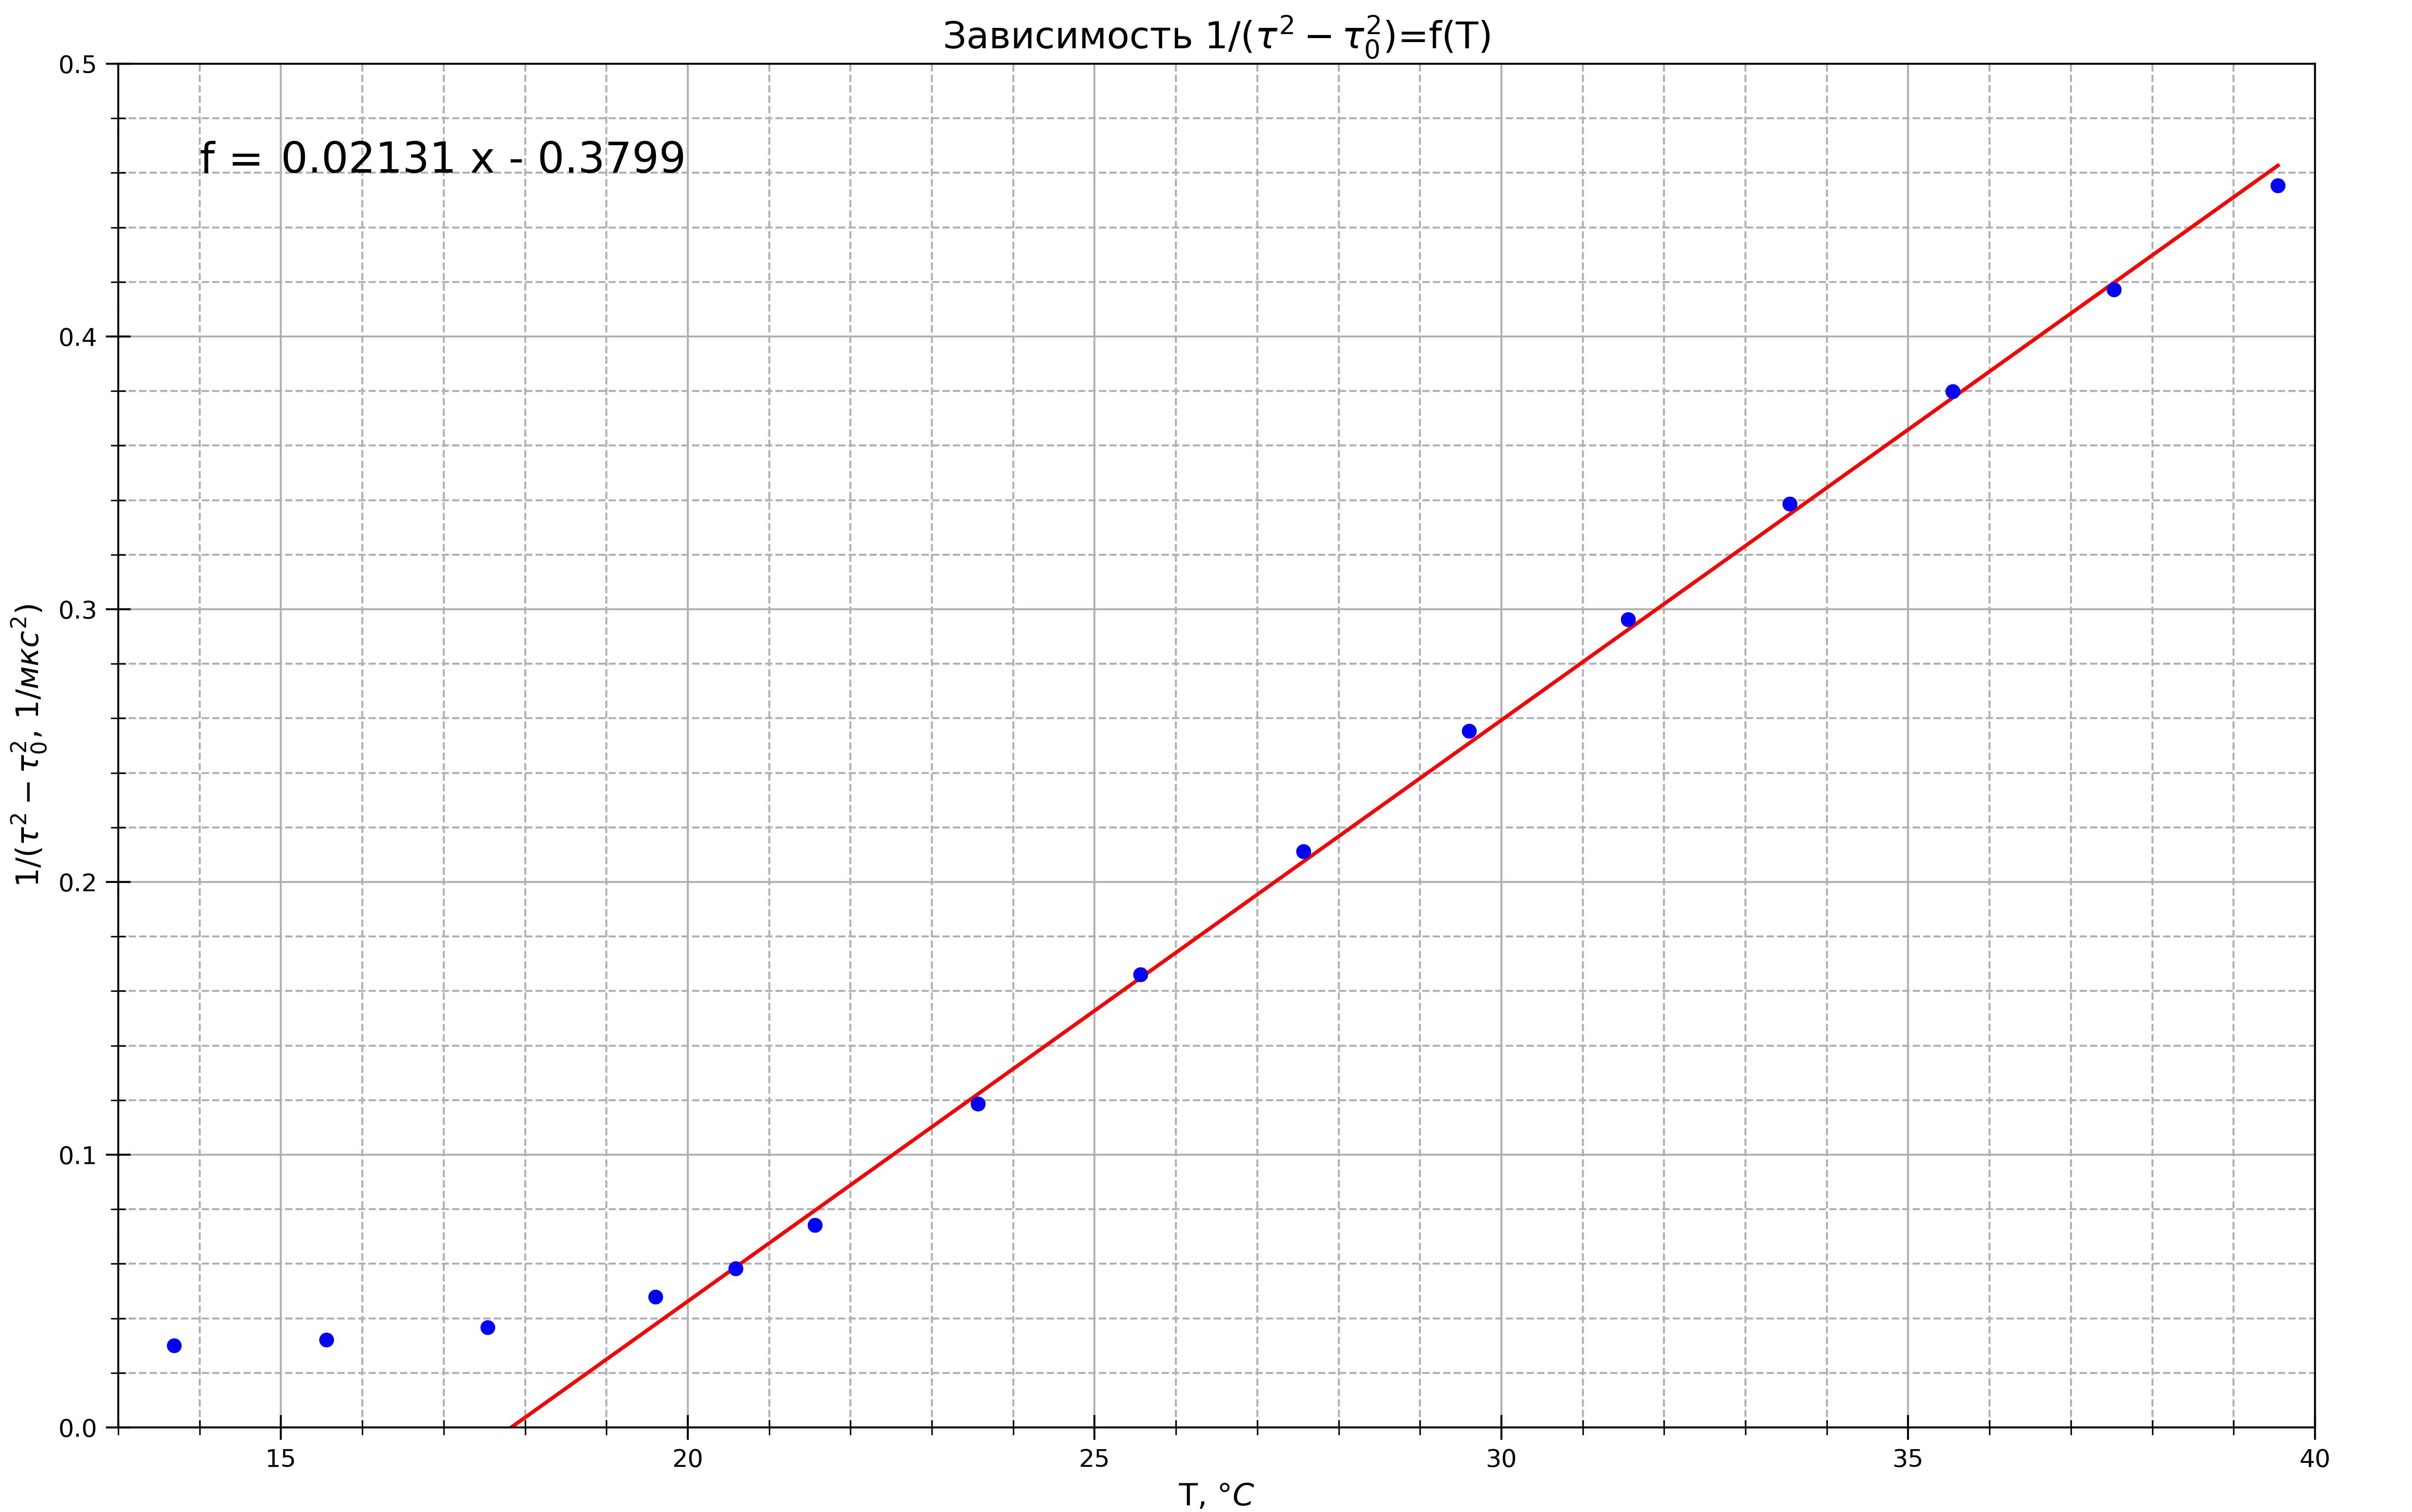
\includegraphics[width=0.9\linewidth]{graph2.png}
\caption{$\frac{1}{\tau ^{2} - \tau _{0}^{2}} = f(T)$}
\label{fig:mpr}
\end{figure}
Мы получили прямую $f = 0,02131\cdot x - 0,3799$. Коэффициент при $x$ равен $0,02131 \pm 0,00016$. Найдём парамагнитную точку Кюри и учтём погрешность МНК.
\begin{center}
    $T_{пт}=17,8 \pm 0,2~\degree C$
\end{center}
\newpage
\subparagraph{3.}Построим график $\tau ^{2} - \tau _{0}^{2} = f(T)$.

\begin{figure}[!h]
\centering
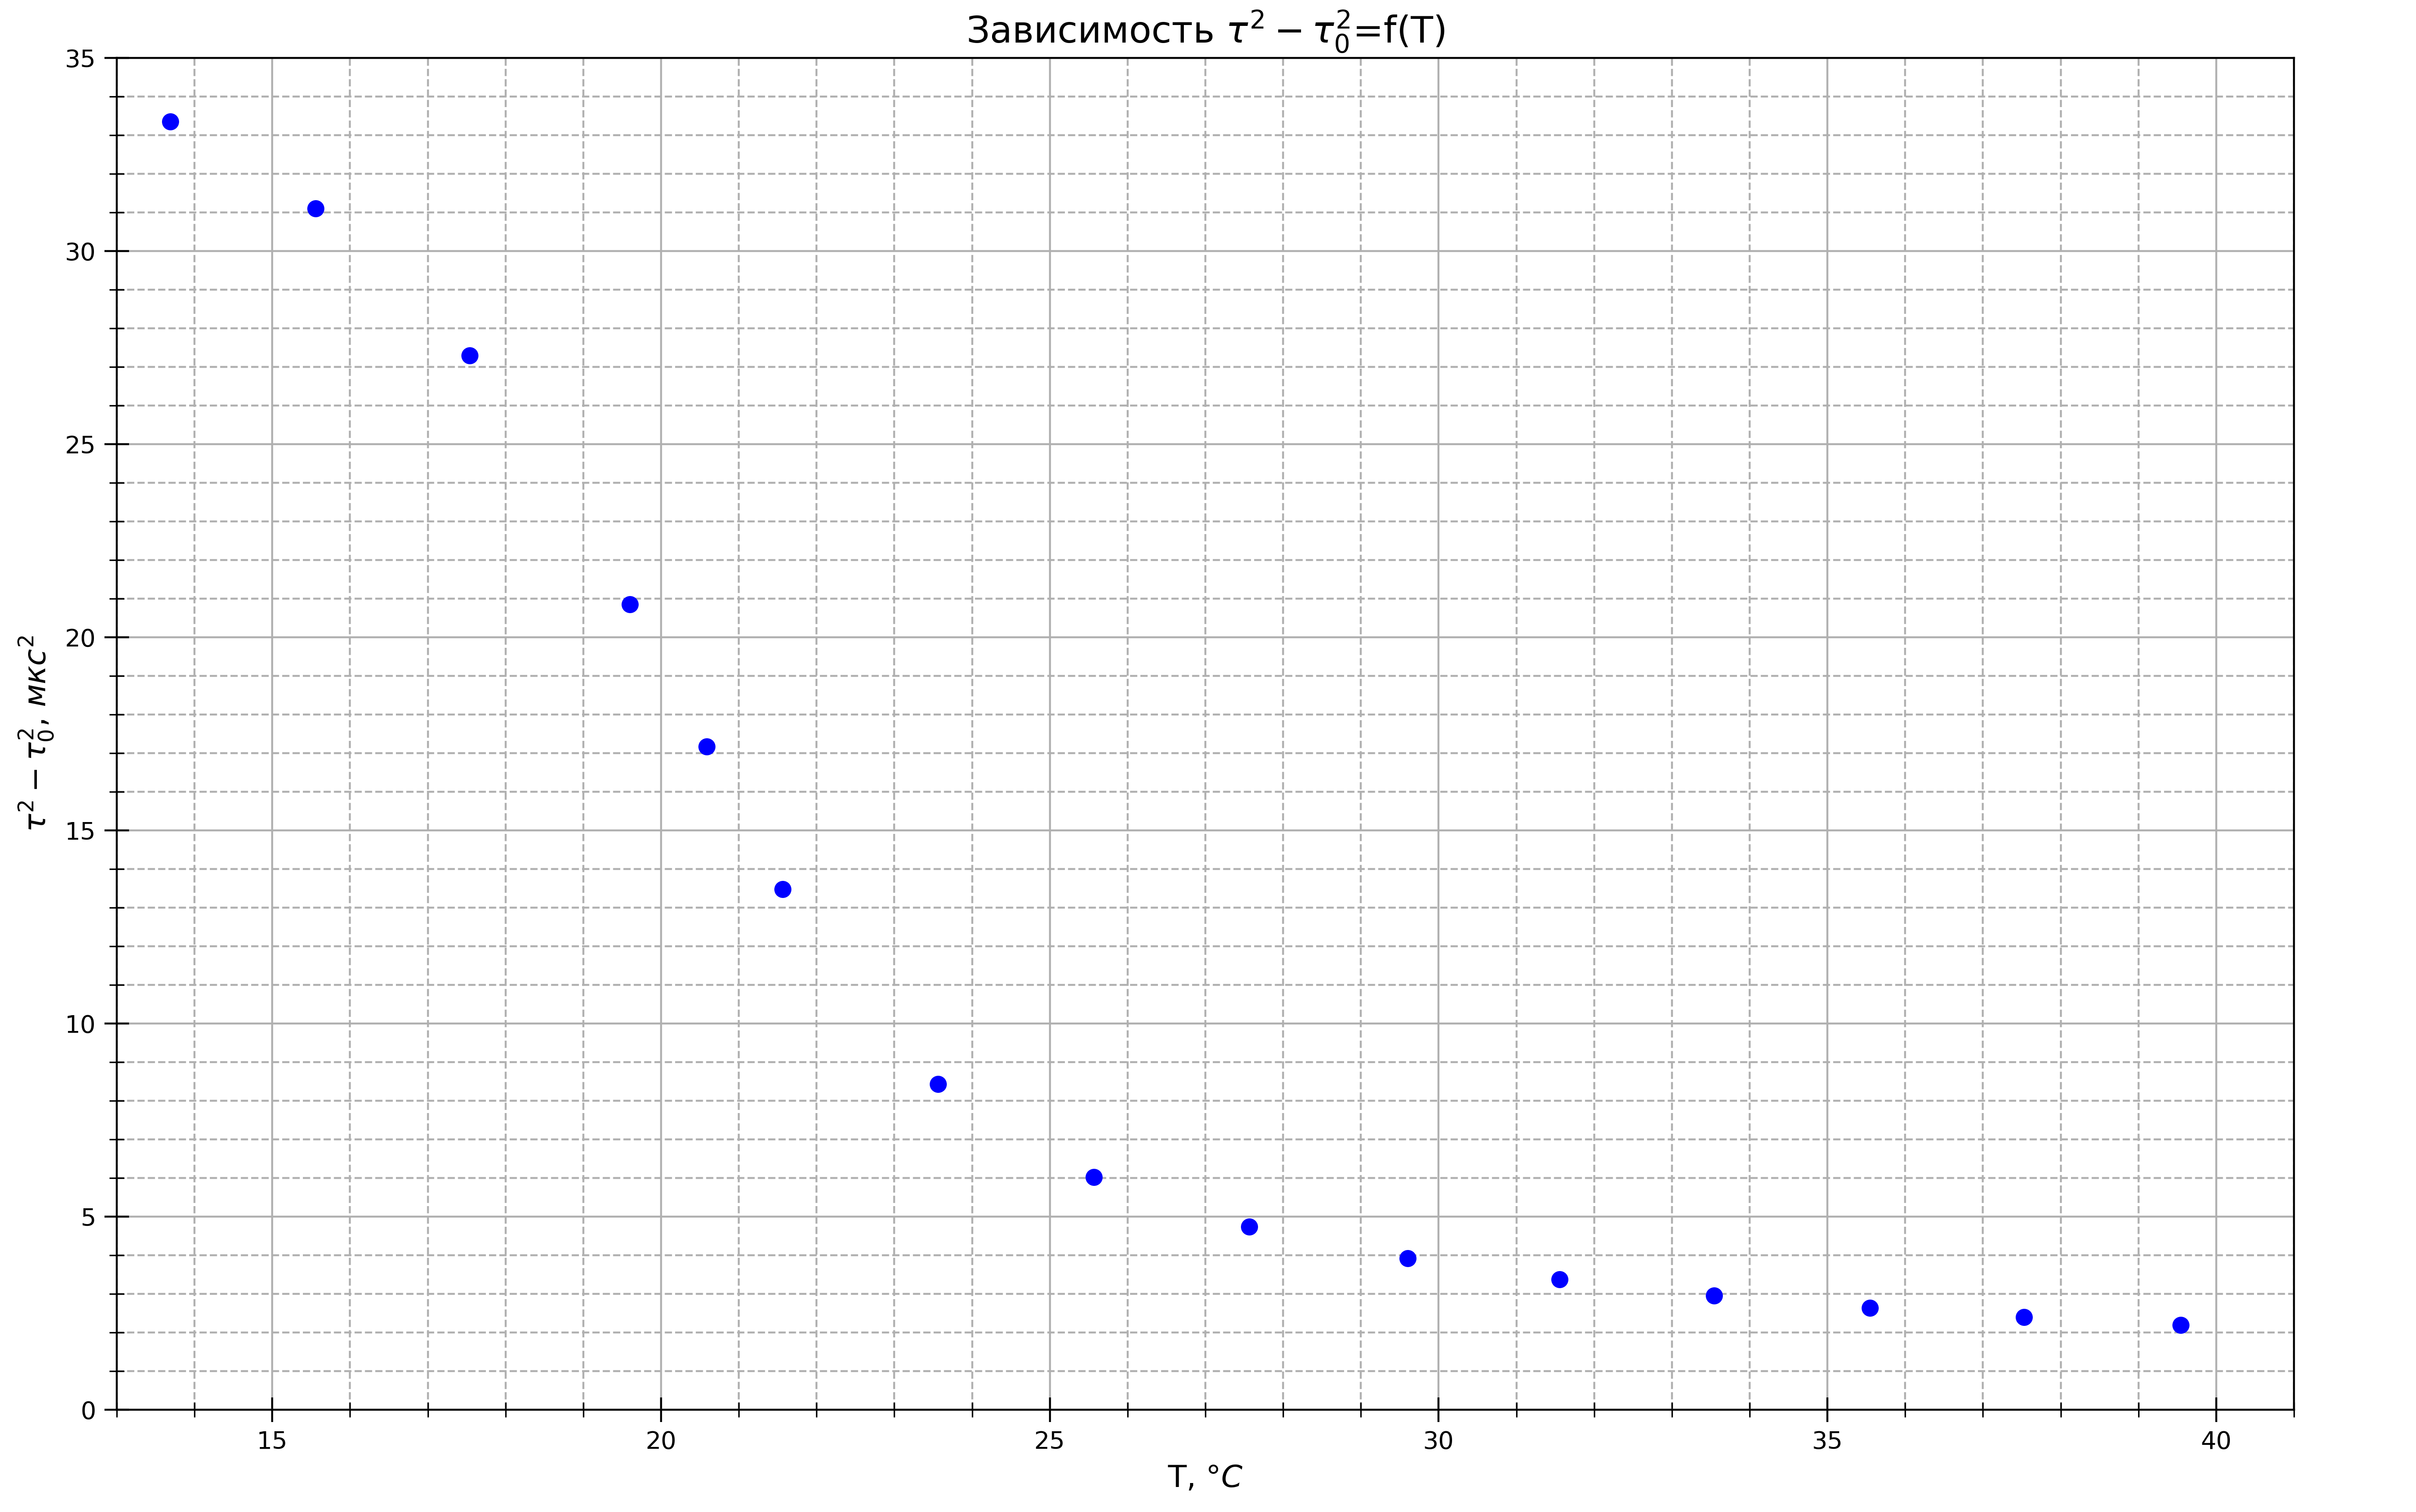
\includegraphics[width=0.9\linewidth]{graph1.png}
\caption{$\tau ^{2} - \tau _{0}^{2} = f(T)$}
\label{fig:mpr}
\end{figure}
В лабораторном практикуме табличное значение точки Кюри гадолиния равна $T_{к}=20~\degree C$. На рис. 3 видно, что при $T>20 \degree C$ магнитная восприимчивость $\chi$ намного меньше.
\paragraph{Вывод:} в ходе работы экспериментально была определена парамагнитная точка Кюри $T_{пт}=17,8 \pm 0,2~\degree C$. Также мы изучили температурную зависимость магнитной восприимчивости ферромагнетика выше точки Кюри.
\end{document}
